% !TeX TS-program = xelatex
% !TeX encoding = UTF-8

\documentclass[11pt, a4paper]{article}
\usepackage[utf8]{inputenc}
\usepackage{graphicx}
% 字体设置
\usepackage{xeCJK}
\setCJKmainfont[BoldFont=SimHei,ItalicFont=KaiTi]{SimSun}
\setCJKmonofont{SimSun}
\setCJKsansfont{SimSun}
% 页面设置
\usepackage{indentfirst}



% 数学记号
\usepackage{amsmath,amssymb,amsthm,amsfonts}
\usepackage{bm}
\DeclareSymbolFont{cmsymbols}{OMS}{cmsy}{m}{n}
%\SetSymbolFont{cmsymbols}{bold}{OMS}{cmsy}{b}{n}
\DeclareSymbolFontAlphabet{\mathcal}{cmsymbols}
% 自定义数学记号在这里
\newcommand{\mat}[1]{\bm{#1}}
\newcommand{\argmax}[1]{\underset{#1}{\operatorname{argmax}}}
\newcommand{\argmin}[1]{\underset{#1}{\operatorname{argmin}}}
\newcommand{\inR}[1]{\in\mathbb{R}^{#1}}
\DeclareMathOperator{\svd}{SVD}


% 算法环境
\usepackage{algorithm}
\usepackage{algorithmic}
\usepackage{eqparbox}
\renewcommand\algorithmiccomment[1]{%
	\hfill\#\ \eqparbox{COMMENT}{#1}%
}
\usepackage{etoolbox}  % patch def of algorithmic environment
\makeatletter
\patchcmd{\algorithmic}{\addtolength{\ALC@tlm}{\leftmargin} }{\addtolength{\ALC@tlm}{\leftmargin}}{}{}
\makeatother
\renewcommand{\algorithmicrequire}{\textbf{输入:}}
\renewcommand{\algorithmicensure}{\textbf{输出:}}


% 杂七杂八
\usepackage{lmodern}
\usepackage[T1]{fontenc}
\usepackage{titlesec}
\usepackage{titling}
\usepackage{verbatim}
\usepackage{float}
\usepackage{enumerate}
\usepackage{enumitem}
\usepackage{amsthm}
\usepackage{graphicx,wrapfig,lipsum}
\usepackage[usenames,dvipsnames]{color}
\usepackage{xcolor}
\usepackage{tikz}
\usepackage{hyperref}
\usepackage{caption}
\usepackage{subfig}
\usepackage{microtype}
\usepackage{cleveref}
\usepackage{textcomp}

\colorlet{inlinkcolor}{green!50!black}
\colorlet{exlinkcolor}{red!50!black}
\hypersetup{
	colorlinks=false,
	frenchlinks=false,
	pdfborder={0 0 0},
	naturalnames=false,
	hypertexnames=false,
	breaklinks,
	colorlinks = true,
	allcolors = inlinkcolor,
	urlcolor = exlinkcolor,
}


% 代码
\usepackage{listings}


%\lstloadlanguages{Matlab}
\lstset{language=Matlab,
	frame=single,                           % single framed
	basicstyle=\small\ttfamily,
	keywordstyle=[1]\color{Blue}\bfseries,  % primitive funs in bold blue
	keywordstyle=[2]\color{Purple},         % args of funs in purple
	keywordstyle=[3]\color{Blue}\underbar,  % user funs in blue with underbar
	stringstyle=\color{Purple},             % strings in purple
	showstringspaces=false,
	identifierstyle=,
	commentstyle=\usefont{T1}{pcr}{m}{sl}\color{DarkGreen}\small,
	tabsize=4,
	% more standard MATLAB funcs
	morekeywords={sawtooth, square},
	% args of funcs
	morekeywords=[2]{on, off, interp},
	% user funcs
	morekeywords=[3]{FindESS, homework\_example},
	morecomment=[l][\color{Blue}]{...},     % line continuation (...) like blue comment
	numbers=left,
	numberstyle=\tiny\color{Blue},
	firstnumber=1,
	stepnumber=1
}


% 环境中文化
\floatname{figure}{\texttt{图}}
\floatname{table}{\texttt{表}}
\floatname{algorithm}{\texttt{算法}}

\theoremstyle{plain}
\newtheorem{theorem}{\texttt{定理}}
\crefname{theorem}{定理}{定理}
\Crefname{theorem}{定理}{定理}

\theoremstyle{plain}
\newtheorem{lemma}{\texttt{引理}}
\crefname{lemma}{引理}{引理}
\Crefname{lemma}{引理}{引理}

\theoremstyle{plain}
\newtheorem{corollary}{\texttt{推论}}
\crefname{corollary}{推论}{推论}
\Crefname{corollary}{推论}{推论}

\theoremstyle{definition}
\newtheorem{definition}{\texttt{定义}}
\crefname{definition}{定义}{定义}
\Crefname{definition}{定义}{定义}

\theoremstyle{remark}
\newtheorem*{remark}{\texttt{备注}}
\crefname{remark}{备注}{备注}
\Crefname{remark}{备注}{备注}

\theoremstyle{definition}
\newtheorem{example}{\texttt{例}}
\crefname{example}{例}{例}
\Crefname{example}{例}{例}

\crefname{equation}{\textsf{公式}}{\textsf{公式}}
\Crefname{equation}{\textsf{公式}}{\textsf{公式}}

\crefname{algorithm}{\texttt{算法}}{\texttt{算法}}
%\Crefname{algorithm}{alg}{alg}

\renewcommand\qedsymbol{$\blacksquare$}	
\renewcommand*{\proofname}{\texttt{证明:}\nopunct}
\usepackage{xcolor}

\newcommand{\T}[1]{\texttt{#1}}
\newcommand{\nl}{\newline}
\newcommand{\red}[1]{\textcolor{red}{#1}}
\newcommand{\blue}[1]{\textcolor{blue}{#1}}
\newcommand{\s}{\footnotesize}

\usepackage{fancyhdr}
\renewcommand{\abstractname}{\large \T{摘  要}}
\usepackage[nottoc,notlof,notlot]{tocbibind} 
\newcommand{\Page}{
	\thispagestyle{fancy}
	\rhead{}
	\chead{\T{“高等数值算法与应用”期末Project报告(2020年秋季学期)}}
}

\pagestyle{fancy}
\fancyhf{}
\chead{\T{“高等数值算法与应用”期末Project报告(2020年秋季学期)}}
\rfoot{\T{第}\thepage\T{页}}
\usepackage{multirow}
\usepackage{multicol}



\begin{document}
	
\title{大规模稀疏矩阵迭代解法研究报告}
\author{\T{郭文韬, 刘志强}}
\date{\T{2021年1月13号}}
\maketitle
\Page

\begin{abstract}
\T{我们探讨了多级低秩修正预条件子(MLR),基于舒尔补的区域分解预条件子(SLR),以及图稀疏化预条件子(feGRASS预条件子)。对于对称正定稀疏矩阵,我们初步比较了MLR, SLR, feGRASS, IChol, 块Jacobi,以及区域分解预条件子在PCG上的性能差异,我们发现MLR和SLR一般可以减少迭代步数,但MLR不一定能减少迭代时间。在更加稀疏的矩阵下,图稀疏化预条件子迭代速度会明显高于其他预条件子,除此之外图稀疏化预条件子的填入元是最少的。对于非对称稀疏矩阵,我们比较了ILU和图稀疏化预条件子在GMRES上的性能差异。我们发现图稀疏化预条件子在迭代步数/时间和填入元方面都明显优于ILU预条件子,但是也存在着稀疏化以后矩阵接近奇异的问题。}
	
\end{abstract}

{\T{关键词:} \T{预条件子}, \T{多级低秩修正}, \T{舒尔补}, \T{区域分解}, \T{图稀疏化}, \T{图切割}
}


\section*{\T{引言}}
% 1
\T{
	矩阵的求解($A x = b$)一般分为直接解法和迭代解法。 对于小规模的矩阵,人们一般采用LU分解(当然也有选主元等增加算法稳定性的方法),Choleskey分解(对于对称正定矩阵)等方法。迭代解法更适用于大规模的稀疏矩阵。 常用的迭代解法有Jacobi迭代,高斯-赛德尔迭代,逐次超松弛法(SOR方法,以及用于对称矩阵的SSOR),预处理共轭梯度(PCG)等方法\cite{Iter}。迭代解法的收敛速度一般难以确保,所以经常需要人为添加“预条件子”来加快收敛速度和解的准确性。常见的预条件子可以被分为三大类\cite{Course}:
}

\begin{gather}
	M^{-1} A x = M^{-1} b \\
	A M^{-1} u = b, \ x = M^{-1} u \\
	M_L^{-1} A M_R^{-1} u = M_L^{-1} b, \ x = M_R^{-1} u
\end{gather}

\T{
	预条件子$M$需要尽可能做到$M^{-1} \approx A^{-1}$来降低迭代矩阵的2-条件数来提高迭代的收敛速度和解的准确性,在实际运用中经常可以和PCG,GMRES等方法有效结合。
}

\T{	
	传统的预条件子有(块)Jacobi预条件子, 高斯-赛德尔预条件子,SOR(SSOR)预条件子,也有给不完全Choleskey分解/不完全LU分解的预条件子。在迭代算法中,块Jacobi迭代适合于并行的实现,但其他的迭代算法未必适合。类似地,我们也希望预条件子的计算也尽可能支持并行。
}

\T{Y. Saad\cite{Course}提到}\T{一些工业界支持并行的预条件子有Schwarz预条件子,基于舒尔补的,以及多级ILU类的预条件子。 在本次project,我们主要探讨了基于舒尔补的预条件子和多级低秩修正的ILU/IC预条件子。}\T{我们也采用了区域分解技术}\cite{MLR}\T{对矩阵进行划分边界/内部节点然后使用metis包做图切割。我们最后也采用了W.Yu, Z.Liu和Z.Fen提出的feGRASS图稀疏化技术\cite{Sparse}来处理非对称稀疏矩阵。}

\section{\T{多级低秩修正(MLR)预条件子方法}}
\subsection{\T{图分割}}
\T{我们知道块Jacobi预条件子$M = \text{diag}(A_{11}, \ldots, A_{nn})$ 易于并行,但假如对对角块做完全分解则消耗内存大,假如做不完全分解迭代步数还是会很高。但我们可以对于$A = \begin{bmatrix} A_{11} & A_{12} \\ A_{21} & A_{22} \end{bmatrix}$, 我们可以选$B = \begin{bmatrix} A_{11} & \\ & A_{22} \end{bmatrix}$, 然后做一个低秩近似使得 $M^{-1} = B^{-1}+LRC$。
}


\begin{figure}[H]
	\label{domain}
	\caption{\T{图分割-以边切割\cite{MLR}}}
	\centering
	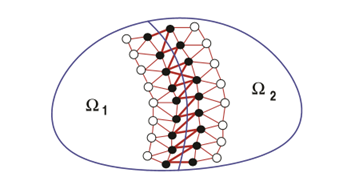
\includegraphics[width=200pt,height=100pt]{graph.png}
\end{figure}

\T{我们先对稀疏矩阵A用Metis\cite{Metis}进行图切割(以边切割\footnote{以边切割是指图切割的时候按边界节点连接的边来划分,如上图所示}),然后将$A$重排序并转换成\eqref{metis_res}的形式\cite{MLR}。}

\begin{equation}
	\label{metis_res}
	\begin{pmatrix}
		\hat{B_{1}} & \hat{F_{1}} & \vline & & \\
		\hat{F_{1}^T} & C_1 & \vline & & -W \\
		\hrulefill & \hrulefill & \vline & \hrulefill & \hrulefill \\
		& & \vline & \hat{B_{2}} & \hat{F_{2}} \\
		& -W^T & \vline & \hat{F_{2}^T} & C_2
	\end{pmatrix}
\end{equation}

\T{设$m_i\ (i = 1, 2)$为区域$\Omega_i$的边界节点的数量。}

\T{其中$\hat{B_i}$和$C_i$对应区域$\Omega_i$的内部/边界节点,$\hat{F_i}$对应内部-边界节点的连接边,$W\in \mathbb{R}^{m_1 \times m_2}$对应区域1和区域2边界节点的连接边。
}

\T{我们分解$W$, 使得$W = X_1 X_2$, 然后引入$E = [0; X_1; 0; X_2^T] \in \mathbb{R}^{n \times m_1}$。}

\T{我们此时可以把$A$改写成以下形式\cite{MLR}。}
\begin{equation} 
	\label{1.a}
	A = B - E E^T, \ B = \begin{pmatrix} B_1 & \\ & B_2 \end{pmatrix}, \ B_i = \begin{pmatrix}
		\hat{B_i} & \hat{F_i} \\ \hat{F_i^T} & C_i + D_i
	\end{pmatrix}
\end{equation}
\T{其中, $D_1 = X_1 X_1^T ,\  D_2 = X_2^T X_2^T$ }

\T{然后根据\textbf{Sherman-Morrison 公式}, 我们可以得到以下等式:}
\begin{equation}
	\label{1.b}
	A^{-1} = B^{-1} + B^{-1}E{\underbrace{(I - E^TB^{-1}E)}_{X}}^{-1}E^TB^{-1} \equiv B^{-1} + B^{-1}EX^{-1}E^TB^{-1}
\end{equation}

\T{我们可以对$B^{-1}E$进行SVD分解(rank-k截断)来低秩近似\cite{MLR}。}
\begin{align}
	\label{1.c}
	\tag*{\T{rank-k低秩近似}}
	B^{-1} E \approx U_k V_k^T
\end{align}

\T{最后,从\eqref{1.b}, \eqref{1.c}我们可以写出以下预条件子\footnote{详细推导过程过程请见\cite{MLR} 第2.2和第3节}。}
\begin{align} 
	\label{1.d}
	\tag*{\T{低秩修正预条件子 }}
	M^{-1} = B^{-1} + U_k H_k U_k^T, \ H_k = (I - U_k^T E V_k)^{-1} 	
\end{align}

\subsection{\T{多级方法}}
\T{我们可以进一步扩展低秩修正预条件子到多级的情况。首先,我们可以将对角块$A_i$写成$B_i - E_i E_i^T, \ B = \begin{pmatrix} B_{i_1} & \\ & B_{i_2} \end{pmatrix}$。 我们可以进一步递归展开$A_i^{-1}$来得到$M_i^{-1}$。}
\begin{gather}
	\begin{aligned}
		M_i^{-1} &\equiv A_i^{-1} = \begin{pmatrix} A_{i_1}^{-1} & \\ & A_{i_2}^{-1} \end{pmatrix} + U_i H_i U_i^T \\
		&\approx B_i^{-1} + U_i H_i U_i^T \\
		&\approx \begin{pmatrix} M_{i_1}^{-1} & \\ & M_{i_2}^{-1} \end{pmatrix} + U_i H_i U_i^T \\
	\end{aligned}
\end{gather}
\T{我们最后可以得到以下多级递推式(MLR)\cite{MLR}:}
\begin{equation}
	\tag*{\T{MLR预条件子递归式}}
	M_i^{-1} = \begin{cases}
		\begin{pmatrix}
			M_{i_1}^{-1}  & \\
			 & M_{i_2}^{-1}
		\end{pmatrix} + U_i H_i U_i^T & \text{\T{假如i不是叶子节点}} \\
	L_i^{-T} L_i^{-1} \, \text{\T{或}} \, L_i^{-T} D_i^{-1} L_i^{-1} & \text{\T{i是叶子节点, 做IC/ILU分解}}
	\end{cases}
\end{equation}

\section{\T{基于舒尔补的低秩修正(SLR)预条件子}}

\T{对于矩阵A,我们可以图切割(用metis做图切割-对边划分,方法和上面MLR的方法一样),并按图切割的结果来重排序。}
\begin{figure}[H]
	\label{SLR-1}
	\caption{SLR-按边划分矩阵\cite{SLR}}
	\centering
	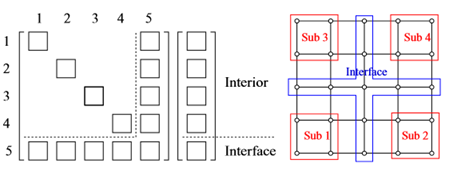
\includegraphics[width=300pt,height=120pt]{SLR.png}
\end{figure}

\T{构造边界方程并求解:}
\begin{gather}
		A \begin{bmatrix}
			x \\ y
		\end{bmatrix} = \begin{bmatrix}
			f \\ g 
		\end{bmatrix} \quad A = \begin{bmatrix}
			B & E \\ F & C
		\end{bmatrix} \\ 
\end{gather}
\T{其中$B = \begin{bmatrix}
		B_1 & & \\
		& \ddots & \\
		& & B_p
	\end{bmatrix}$代表区域$1...p$的内部节点,$F = [F_1 \cdots F_p],\ E = [E_1; \cdots; E_p]$代表区域$1...p$的内部-边界节点连接边,$C$代表边界节点}

\T{我们知道}
\begin{gather}
		\begin{cases}
			x = B^{-1}(f - E y) \\
			(C - F B ^{-1} E) y = g - F B^{-1} f
		\end{cases}
\end{gather}

\T{然后构造舒尔补$S = C - F B^{-1} E$需要求解 \red{$s$} 次$B$。 我们此时需要构造一个$\hat{S}$来近似$S$, 然后得到预条件子:}

\begin{equation}
	\tag{\T{SLR预条件子}}
	M = \begin{pmatrix}
		I & \\ F B^{-1} & I
	\end{pmatrix} \begin{pmatrix}
		B & E \\ & \hat{S}
	\end{pmatrix}
\end{equation}

\T{假如我们用$C^{-1}$ 来近似 $S^{-1}$\footnote{\cite{SLR}的第5节有更详细的探讨},我们可以得到\underline{区域分解(DD)的预条件子}, 此时预条件子求解仅需求解 \red{2} 次$B$。 另一种做法是对$S$做低秩近似\cite{SLR}:}
\begin{equation}
	\label{SLR-2}
	S^{-1} \approx C^{-1} + LRC
\end{equation}
\T{这时我们可以引入矩阵$H$做谱分解\cite{SLR}。}

\T{设一个矩阵$H$满足:}
\begin{equation}
	H = L^{-1}E^TB^{-1}EL^{-T} = UDU^T, \quad U\text{\T{为酉矩阵}}, \ D = \text{diag}(\lambda_1, \ldots, \lambda_s)
\end{equation}
	
\T{则$S$满足\cite{SLR}} 
\begin{equation}
	S = L(I - H)L^T
\end{equation}

\T{然后我们可以近似$S^{-1}$\cite{SLR}。}	

\begin{gather}
	\begin{aligned}
		S^{-1} &= L^{-T} (I - H)^{-1}L^{-1} \\ &= L^{-T} U (I - D)^{-1} U^T L^{-1} \\
		&\approx L^{-T} U (I - \tilde{D})^{-1} U^T L^{-1} ,\quad \tilde{D} = \text{diag}(\tilde{\lambda_1}, \ldots, \tilde{\lambda_s}) \\
		&\approx C^{-1} + L^{-T} U[(I - \tilde{D})^{-1} - I]U^TL^{-1}
	\end{aligned}
\end{gather}

\T{R. Li, Y. Xi和Y. Saad中提出\cite{SLR}了以下几种近似谱分解算法,不同的近似谱分解算法所带来的$S \tilde{S}^{-1}$的谱范数不同以及所带来的收敛性也不同。}
\begin{multicols}{2}
	\begin{itemize}
		\item
		\begin{equation}
			\nonumber
			\tilde{\lambda_i} = \begin{cases}
				\lambda_i \quad &\T{ 假如 } i \leq k \\
				0 \quad &\T{ 其他情况}
			\end{cases}
		\end{equation}
		
		\item
		\begin{equation}
			\nonumber
			\tilde{\lambda_i} = \begin{cases}
				1 \quad & \T{ 假如 } i \leq k \\
				1 - \lambda_i \quad & \T{ 其他情况}
			\end{cases}
		\end{equation}
		
		\item
		\begin{equation}
			\nonumber
			\tilde{\lambda_i} = \begin{cases}
				1 - (1 - \lambda_i) / \epsilon \quad & \T{ 假如 } i \leq k \\
				0 \quad & \T{ 其他情况}
			\end{cases}
		\end{equation}
	\end{itemize}
\end{multicols}

\T{但是我们最后采用的是用Matlab中eigs命令直接取$S$的前$k$个最大的特征值(我们测试用的$k$是20)。}


\section{\T{基于图稀疏化技术(feGRASS)的预条件子}}
% .7

\T{我们知道矩阵$A$可以分成对角矩阵$D$,上对角,下对角矩阵$L$、$U$。}
\begin{equation}
	A = D + L + U
\end{equation}

\T{我们可以将$L$和$U$分别看成两个无向图$\tilde{L}$、$\tilde{U}$, 然后分别采用无向图稀疏化技术\cite{Sparse}。}
\T{对于负数边,我们将其权值处理为一个极小的正数。}
\T{我们可以得到以下预条件子\ref{feGRASS}。}
\begin{align}
		\label{feGRASS}
		\tag{图稀疏化预条件子}
		M = D + \tilde{L} + \tilde{U}
\end{align}





\section*{\T{实验与讨论}}
% 1
\T{因为不同的预条件子使用条件不同,我们分开用对称正定矩阵和一般非对称矩阵进行了测试,测试样例可以在\href{http://sparse.tamu.edu/}{SuiteSparse Matrix Collection}可以找到\cite{Test}。}
\begin{itemize}
	\item[1] 对称正定矩阵
	
	\T{我们用对称正定矩阵作为输入,用PCG求解速度/每行填入数量测试了六种预条件子方法Ichol、feGRASS、Block Jacobi、DD type、MLR、SLR\footnote{Block Jacobi、DD type、MLR、SLR方法都划分为8个子区域,子区域内部使用Ichol}。}
	
	\begin{center}
		\begin{table}[H]
			\caption{\T{测试(对称正定)矩阵参数}}
			\begin{center}
				\begin{tabular}{ c|c|c|c}
					\T{矩阵名字} & size & NNZ (\T{百分比}) & \T{2-条件数} \\
					\hline
					Dubcova2 & 65025 * 65025 & 1030225 (.024\%) & 1.04e+04 \\
					\hline
					Dubcova3 & 146689 * 146689 & 3636643 (.017\%) & 1.15e+04 \\
					\hline
					Ecology2 & 999999 * 999999 & 4995991 (.0005\%) & 6.66e+07 \\
					\hline
					Thermal1 & 82654 * 82654 & 574458 (.0084\%) & 4.96e+05	\\
					\hline
					Thermal2 & 1228045 * 1228045 & 8580313 (.00057\%) & 7.48e+06 \\
					\hline
					Apache2 & 715176 * 715176 & 4817870 (.00094\%) & 5.32e+06 \\											
				\end{tabular}
			\end{center}
		\end{table}
	\end{center}
	
	\begin{figure}[H]
		\caption{\T{对称正定矩阵实验结果}}
		\centering
		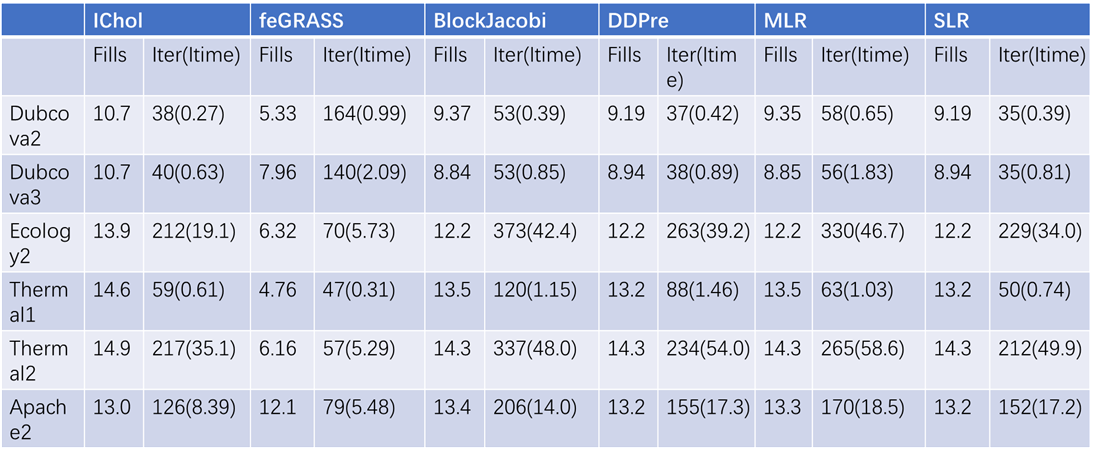
\includegraphics[width=350pt,height=160pt]{SPD_res.png}
	\end{figure}


	\T{经过测试	\footnote{\T{测试结果中Fill是指平均每行的填入元}},我们可以发现}
	\begin{itemize}
		\item \T{相比于块-Jacobi预条件子,低秩修正预条件子确实能降低迭代步数,但MLR是否能缩短迭代时间存疑。}
		
		\item \T{SLR一般比MLR迭代速度要更快,但填入元SLR和MLR没有很明显的差异。}
		
		\item \T{对于相对稠密的矩阵(Dubcova2/Dubcova3), feGRASS技术迭代步数会显著高于其他预条件子, 但对于更加稀疏的矩阵,feGRASS技术的迭代步数/速度会明显快于其他预条件子。}
		
		\item \T{feGRASS的填充元是上面6种预条件子中最少的。}
	\end{itemize}
	
	
	
	\item[2] 一般非对称矩阵
	
	\T{对于ILU、feGRASS方法,我们使用一般非对称矩阵作为输入源并使用GMRES求解(restart = 10)。}
	
	\begin{figure}[H]
		\caption{\T{一般非对称矩阵实验结果}}
		\centering
		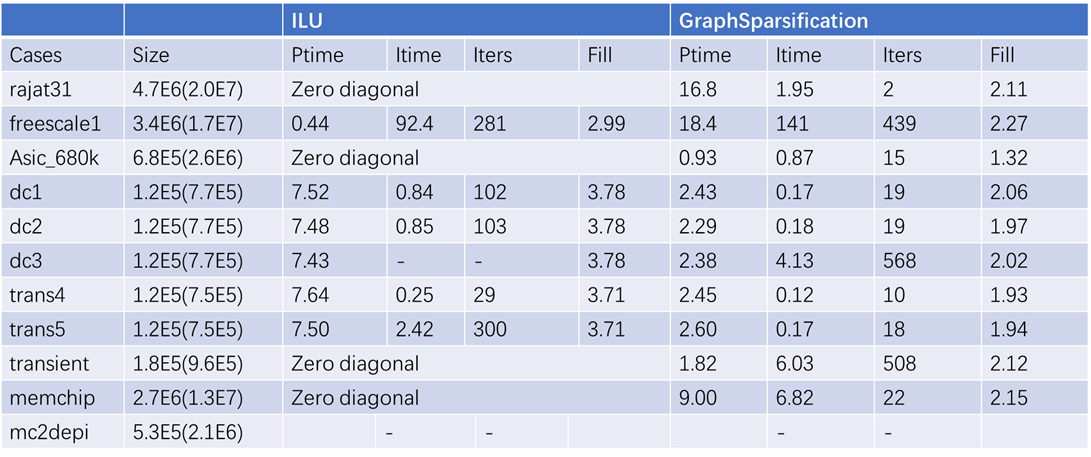
\includegraphics[width=350pt,height=180pt]{normal.png}
	\end{figure}
	\T{经过测试,我们可以发现}
	\begin{itemize}
		\item \T{非对称矩阵稀疏化(feGRASS)方法迭代时间/步数一般优于ILU,且每行填入元明显少于ILU,但是也存在着稀疏化以后矩阵接近奇异的问题。}
		\item \T{Matlab ILU命令可能无法得到分解结果。}
	\end{itemize}

\end{itemize}




\section*{\T{总结}}
\T{我们这一次期末project主要学习并比较了几种预条件子。针对对称正定矩阵的预条件子,我们编程实现了MLR预条件子,SLR预条件子以及基于图稀疏化技术的预条件子,然后我们也对其性能做了一个初步的研究比较,但目前我们的实现还比较原始,未能实现完全并行计算。在对称正定矩阵上,feGRASS的填入元可以明显减少,但图稀疏化预条件子的迭代时间/步数依赖于原始矩阵的稠密性。SLR在迭代时间/步数一般优于MLR,但在填入元上MLR和SLR结果相近。MLR在迭代步数上一般优于feGRASS,但MLR不一定能缩短迭代时间。 针对非对称矩阵,我们发现图稀疏化方法在迭代时间/步数上一般优于ILU,但是也存在着稀疏化以后矩阵接近奇异的问题。
}
\T{未来我们会关注于MLR和SLR的并行化实现并尝试针对较为稠密的矩阵进一步优化图稀疏化技术。}


\renewcommand{\refname}{\T{参考文献}}
\bibliographystyle{plain}
\bibliography{参考文献.bib}

\end{document}

